\section{Software Implementation}
\fred is part of the \sksurgery\cite{PMID:32436132} family of libraries. In common with \sksurgery the majority of \fred is implemented in Python. Python was chosen as it combines sufficient features for clinical
applications, whilst remaining easy enough for students to learn and contribute to. A key design goal of 
\sksurgery is to keep individual libraries compact and orthogonal\cite{pragmaticprog}, simplifying dependency structures. Based on 
analysis using cloc\footnote{\href{https://github.com/AlDanial/cloc}{https://github.com/AlDanial/cloc} [v1.82]} \fred consists of 802 lines of Python 
code. The user interface is implemented in HTML5 and JavaScript, enabling multiple simple deployment 
options. Again, using cloc, there are 561 lines of HTML5 and JavaScript. These numbers are similar to the other \sksurgery libraries which typically have around 2000 lines of code \cite{PMID:32436132}. In comparison, this paper consists of around 400 (CHECK ME) lines of Latex code.

Figure \ref{fig:dependencies} shows the direct dependencies of \fred. The key functional dependency is
\core\cite{matt_clarkson_2020_3965731}. \core implements matched point based registration \cite{Arun1987} together 
with the calculation of expected \gls{FLE} and \gls{TRE} (equations 10 and 31 from Fitzpatrick et al.\cite{Fitzpatrick1998}). Flask\footnote{\href{https://palletsprojects.com/p/flask/}{https://palletsprojects.com/p/flask/}  [v1.1.2]} provides the web application framework 
to enable the browser based user interface to communicate with the Python based back end. The user
interface communicates with the back end with a series of {POST} requests. All state information is stored in the 
browser front end, allowing the back end to remain stateless, simplifying deployment. 
Including the Google Cloud FireStore API\footnote{\href{https://pypi.org/project/google-cloud-firestore/}{https://pypi.org/project/google-cloud-firestore/} [v2.0.1]} 
enables the optional storage of results in a remotely hosted database. Plotting functionality is implemented
using Chart.js\footnote{\href{https://www.chartjs.org/}{https://www.chartjs.org/} [v2.9.4]}

\begin{figure}
	\begin{center}
	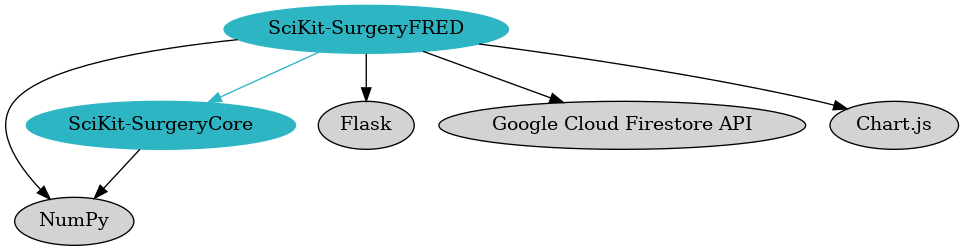
\includegraphics[width=0.7\linewidth]{dependency_graph.eps}
		\caption{\label{fig:dependencies}Software dependencies of SciKit-SurgeryFRED. The registration algorithms and statistical measures of {TRE} are imported from SciKit-SurgeryCore and are shared with clinical applications built on SciKit-Surgery. The user interface is a Flask based web application, using Chart.js for plotting functionality.}
	\end{center}
\end{figure}

In common with the rest of \sksurgery \fred utilises extensive testing and software process \cite{1398621} to 
ensure the application is robust, reusable, and sustainable\cite{VENTERS2018174}. Change control and issue tracking is managed
on GitHub\footnote{\href{https://github.com/UCL/scikit-surgeryfred}{https://github.com/UCL/scikit-surgeryfred}} and continuous integration is managed using
GitHub Actions \footnote{\href{https://github.com/UCL/scikit-surgeryfred/actions}{https://github.com/UCL/scikit-surgeryfred/actions}}.

\subsection{Availability and Usage}
For those who want to quickly try \fred out, we currently maintain a running instance hosted at \href{https://scikit-surgeryfred01.ew.r.appspot.com/}{https://scikit-surgeryfred01.ew.r.appspot.com/}. This should be accessible from most modern web browsers.

If you want to run a locally hosted instance, or modify the code for your needs, you can download the source code. \fred is entirely open source software, the latest version of which can be obtained from Github. Alternatively, archived releases can be retrieved via Zenodo\cite{stephen_thompson_2020_4314971}.

\begin{lstlisting}[language=bash]
	git clone https://github.com/UCL/scikit-surgeryfred
\end{lstlisting}

Once installed the dependencies can be installed on a local virtual machine using tox. The application can then be run with as follows. This should output a web address that you can open in a browser to run the software. 

\begin{lstlisting}[language=bash]
	cd scikit-surgeryfred
	tox
	source .tox/py37/bin/activate
	python main.py
\end{lstlisting}

